\chapter{Fundamentos\label{chap:FundamentacaoMatematica}}

% Resumo opcional. Comentar se não usar.
Esta seção introduz os conceitos por trás das técnicas utilizadas no sistema
de animação computacional proposto neste trabalho. O objetivo deste capítulo 
é introduzir o necessário da teoria das técnicas utilizadas, 
para que se entenda as propriedades dosresultados obtidos. A aplicação 
consiste do encadeamento de diversas técnicas oriundas dos domínios de 
Visão Computacional, Geometria Computacional e Filtragem Digital. Como frequentemente
acontece, as técnicas de Visão Computacional muitas vezes empregam conceitos de 
Aprendizado de Máquina. 


\section{Definições Básicas}

\begin{itemize}
\item Imagem

Uma imagem pode ser definida como uma função bidimensional, $\mathpzc{f}(x,y)$,
onde $x$ e $y$ são coordenadas espaciais e a amplitude de $\mathpzc{f}$ em
qualquer par de coordenadas $(x,y)$ é dita a intensidade ou intensidade de cinza
da imagem naquele ponto. Quando $x$, $y$ e o os valores de intensidade de
$\mathpzc{f}$ são todos finitos e discretos, diz-se que a imagem é uma uma
imagem digital. Uma imagem digital é composta de um número finito de elementos,
cada um destes possuindo um valor e uma localização particular. Estes elementos
são mais comumente chamados de pixeis \cite{gonzalesDigitalImageProc}.

\item Sequência de Imagens

Uma sequência de imagens é uma função tridimensional $\mathpzc{h}(x,y,t)$ que
possui uma ou mais imagens $\mathpzc{f}(x,y)$ tomadas em instantes de tempo
discretos $t$ \cite{def:imageSequence}.

\item Rastreamento

Rastreamento é o problema de inferir o movimento de um objeto dada uma sequência
de imagens. Em um problema típico de rastreamento, tem-se um modelo para o
movimento do objeto e um conjunto de medidas oriundas de uma sequência de
imagem. Não é garantido que essas medidas sejam relevantes, podendo elas conter
informação de outros objetos que não o objeto de interesse
\cite{computer-vision-modern-approach-forsithy}.

\end{itemize}


\section{Ajuste de Modelo Deformável}

Ajuste de Modelo Deformável é o problema de ajustar os parâmetros de um modelo
paramétrico a uma imagem de forma que os pontos chaves correspondam com
localizações do objeto de interesse. É uma tarefa difícil uma vez que envolve
uma otimização em um espaço de alta dimensão, no qual a forma de um objeto pode
variar drasticamente entre instâncias do objeto devido a condições de
iluminação, ruído na imagem, resolução e fontes intrínsecas de variabilidade
\cite{saragih2011deformable}.

Ainda segundo \cite{saragih2011deformable}, uma das abordagens mais proeminentes
para o problema consiste em modelar um objeto utilizando observações
espaço-temporalmente coerentes de imagens locais (\textit{image patches})
centradas nos pontos de interesse dentro do objeto. Nesta abordagem, assume-se
que os \textit{patches} são condicionalmente independentes uns dos outros para
fins computacionais e de generalização da técnica. Os detectores locais são
tipicamente aprendidos, a partir de imagens marcadas de treinamento, para cada
ponto proeminente do objeto.

A Figura \ref{fig:pontos-de-interesse} mostra pontos de interesse que podem ser
utilizados em um modelo deformável para a face humana.

Devido ao pequeno suporte destes detectores e a alta variabilidade de aparência
nos dados de treinamento, estes detectores locais estão fadados à ambiguidade
\cite{saragih2011deformable}. 

\begin{figure*}[!htb]
   \centering
\begin{tabular}{cc}
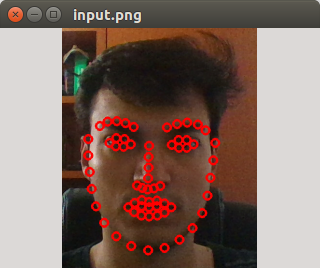
\includegraphics[width=0.4\linewidth]{./figs/sample-detection.png}&
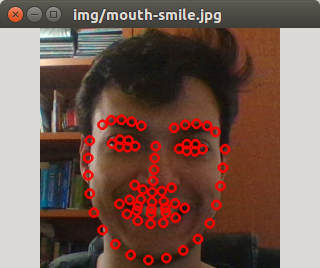
\includegraphics[width=0.4\linewidth]{./figs/sample-detection-2.png}
\end{tabular}
    \caption{Exemplo de regiões de interesse que devem ser marcadas em uma imagem.}
    \label{fig:pontos-de-interesse}
\end{figure*}

\subsection{Ajuste de Modelo Deformável por Deslocamento Regularizado de Média de Pontos Chaves}

O ajuste de modelo deformável por Deslocamento Regularizado de Média de Pontos
Chaves, do inglês \nomenclature{RLMS}{\textit{Regularized Landmark
Mean-Shift}}{\textit{Regularized Landmark Mean-Shift} (RLMS) é uma técnica que
trata o problema de ajuste de modelo deformável empregando sinergicamente as
informações de cada detector local não paramétrico dos pontos proeminentes
\footnote{Ao longo do texto os termos `pontos chave', `pontos proeminentes',
`pontos de interesse' e `marcadores' são sinônimos e referem-se ao conjunto de
pontos rastreados do modelo deformável.} , enquanto limita o efeito de suas
ambiguidades ao ajustar os parâmetros do modelo deformável.

Como é visto a seguir, o modelo deformável paramétrico consiste em um conjunto
de pontos chaves do objeto de interesse. Para cada um desses pontos chaves, o
RMLS utiliza um detector treinado independentemente dos demais. Treiná-los assim
é mais fácil, mas os detectores aprendidos são ruidosos e muitas vezes produzem
resultados ambíguos. O RMLS é uma técnica que permite utilizar as informações de
todos os outros rastreadores para detectar a posição de um ponto proeminente e
não só o rastreador que foi treinado para aquele ponto em específico. Em um
problema de detecção facial, por exemplo, pode-se pensar que se o rastreador
para nariz está em dúvida sobre qual de dois pontos é, mais certamente, o centro
de um nariz, ele pode utilizar informação dos rastreadores dos olhos e da boca
para escolher qual dos dois pontos melhor representa o nariz. 

O exemplo anterior deve ser entendido como uma motivação para a utilização
sinérgica de rastreadores e não mais do que isso. O RLMS é uma técnica de
propósito geral e não assume nenhuma forma para o modelo ou mesmo requer que a
forma como os pontos se arranjam seja informada explicitamente como entrada. O
RLMS aprende conformações prováveis para o conjunto de pontos a partir de dados
de treinamento e poderia ser utilizado tanto para detectar pontos da face humana
como pontos no contorno de um carro. A única diferença seriam os dados de
entrada e, consequentemente, as matrizes aprendidas no processo. 

Quando requerido para ajustar o modelo paramétrico a uma imagem de entrada,
pode-se dizer simplificadamente que o RMLS tentará buscar na imagem de entrada
uma combinação das configurações com as quais ele já foi familiarizado. Como em
muitos outros métodos de Aprendizagem de Máquina, a busca pelos parâmetros que
melhor se adequam é realizada por meio de um processo de otimização de uma
equação de probabilidade. Como parte do objetivo desta fundamentação teórica,
alguns detalhes do RLMS serão apresentados.



\subsection{Modelo de Distribuição de Pontos}

Essa seção especifica o modelo paramétrico utilizado pelo RLMS. O Modelo de
Distribuição de Pontos, do inglês \nomenclature{PDM}{\textit{Point Distribution
Model}} \textit{Point Distribution Model} (PDM), propõe que o objeto a ser
entendido deve ser caracterizado como um conjunto de pontos chaves
bidimensionais no domínio da imagem. O PDM modela linearmente variações de forma
não-rígidas e as compõe com uma transformação rígida global, colocando o i-ésimo
ponto de interesse $\bm{v_i}$ em:

\begin{equation}
 \bm{v_i} = s \bm{R} ( \bm{v}_{i,0} + \bm{\Phi}_i \bm{q}) \bm{t}
\label{eq:PDM-equation}
\end{equation}
 
onde $\mathbf{p}=\{s,\bm{R},\bm{t},\bm{q}\}$ denota os parâmetros do modelo e
consiste do fator de escala $s$, da matriz de rotação $\bm{R}$, do vetor de
translação $\bm{t}$ e de um conjunto de parâmetros não rígidos $\bm{q}$. É esse
conjunto $\mathbf{p}$ que deve ser calculado ao ajustar o modelo a uma imagem
dada, todos os outros termos da equação podem ser previamente calculados em um
processo conhecido como treinamento.  Na Equação \ref{eq:PDM-equation}
$\bm{v_{i,0}}$ denota a posição neutra do $i$-ésimo ponto de interesse e
$\bm{\Phi_i}$ é uma submatriz da base de variações previamente aprendida
pertinente ao $i$-ésimo ponto de interesse.  Nesta equação o termo $\bm{\Phi}_i
\bm{q}$ corresponde à transformação não rígida e os outros termos à
transformação rígida. Nota-se que o modelo consiste de \textbf{uma transformação
rígida aplicada a uma transformação não rígida}. Parte da riqueza do modelo está
na transformação não rígida, que é apresentada mais a fundo a seguir.

O vetor parâmetros não rígidos $\bm{q} \in \realnumbers ^d$ indica o peso com o
qual cada uma das $d$ possíveis transformações não-rígidas influencia o
posicionamento do ponto chave em questão no quadro considerado. O número $d$
deve ser fixado e é referenciado na literatura como a dimensão do PDM. A matriz
$\bm{\Phi}$ contém as $d$ deformações possíveis para cada um dos $K$ pontos de
interesse e a matriz $\Phi_i$ é a submatriz que contém as deformações possíveis
para o $i$-ésimo ponto de interesse.

As constantes $v_{i,0}$ e $\Phi_i$ devem ser aprendidas a partir de um conjunto
de dados de treinamento. O conjunto de dados de treinamento consiste em uma
série de imagens anotadas onde todos os $K$ pontos do PDM foram
\textbf{manualmente} marcados. A partir dessas imagens é possível conhecer as
principais maneiras com que o modelo de pontos aparece deformado na imagem. A
técnica com a qual aprende-se a matriz $\bm{\Phi}$ é a Análise de Componentes
Principais.

Finalmente, nota-se que a Equação \ref{eq:PDM-equation} define $\mathbf{v}_i$
como função de $\mathbf{p}$. A seguinte expansão em série de Taylor é utilizada
para aproximar os valores $\mathbf{v}_i$ em torno de um ponto $\mathbf{v}_i^c$:

\begin{equation}
\mathbf{v}_i \approx \mathbf{v}_i^c + \mathbf{J}_i \Delta \mathbf{p}
\label{eq:alg2}
\end{equation}


\subsection{Análise de Componentes Principais}

A técnica de Análise de Componentes Principais, do inglês
\nomenclature{PCA}{\textit{Principal Components Analysis}} \textit{Principal
Components Analysis} (PCA), é comumente utilizada para reduzir a dimensionalidade
de um conjunto de vetores de características. Um vetor de características é
simplesmente um vetor cujas componentes representam características de um
objeto.  A entrada para a técnica consiste de um conjunto $\mathcal{D}$ de $N$
vetores $D$-dimensionais e a saída é um outro conjunto $D_{PCA}$ de $N$ vetores
$L$-dimensionais. A técnica reduz a dimensionalidade dos dados quando $L < Q$. A
PCA permite isso ao reescrever cada elemento $\bm{v}$ de $D$ como uma combinação
linear de $L$ vetores $D$ dimensionais $\{ \mathbf{w}_1, \mathbf{w}_2, \cdots,
\mathbf{w}_L\}$.  Os pesos $\{z_i\}_{i=1}^L$da combinação se tornam as $L$
componentes do vetor $\mathbf{z} \in \mathcal{D}_{PCA}$. Se a transformação for
perfeita, é possível recuperar unicamente o vetor $\mathbf{v}$ apartir de
$\mathbf{z}$, mas esse não é o caso comum. Em geral a diminuição de dimensão
implica em perda de dados e é possível medir o erro da aproximação. 

Seja $\mathbf{z} = (z_1, z_2, \cdots, z_L)$ um elemento de $D_{PCA}$, uma
estimativa $\mathbf{\hat{v}}$ do vetor $\mathbf{v}$ de $D$ que gerou
$\mathbf{z}$ por meio da transformação é

\begin{equation}
\mathbf{\hat{v}} = z_1 \mathbf{w}_1 + z_2 \mathbf{w}_2 + \cdots + v_L \mathbf{w}_L
\end{equation}

na qual os vetores $w_i, i = 1 \cdots L$ são os vetores base aprendidos pela
PCA. O erro quadrático da transformação é dada por

\begin{equation}
erro_i = ||(\mathbf{\hat{v}}_{i} - \mathbf{v}_i)||^2
\end{equation}

E o erro quadrático médio (a função custo a ser otimizada) para o conjunto de
dados de aprendizagem $\mathcal{D}$ de N elementos $\mathbf{v_i}$ é

\begin{equation}
J(\mathbf{W}, \mathbf{Z} ) = \frac{1}{N}\sum_{i=1}^N ||\mathbf{\hat{v}}_{i} - \mathbf{v}_i||^2
\end{equation}

Onde $\mathbf{W}$ é a matriz obtida concatenado-se os vetores $\mathbf{w}_i$ e
$\mathbf{Z}$ a matriz obtida concatenando-se os $\mathbf{z}_i$. Se $L = D$ então
$E_{total} = 0$ e, geralmente, se $L < D$, $E_{total} > 0$.  Além disso, os
vetores $\mathbf{w}_i$ devem ser ortonormais.

A solução ótima para o problema é conhecida e é encontrada fazendo-se
$\mathbf{W} = \mathbf{V}_L$, onde $\mathbf{V}_L$ contém os L autovetores com
maiores autovalores da matriz empírica de covariância dada por 

\begin{equation}
\hat{\mathbf{\Sigma}} = \frac{1}{N}\sum_{i=1}^{N} \mathbf{v_i}\mathbf{v_i}^T
\end{equation}

Além disso, os $\mathbf{z_i}$ podem ser escritos como $\mathbf{z}_i =
\mathbf{W}^T \mathbf{v}_i$ \cite{machine-learning-book}. Para referências
futuras, nota-se o autovalor associado ao autovetor $\mathbf{w}_i$ por
$\lambda_i$.

A redução de dimensionalidade obtida pela PCA é valiosa por si só, tornando
alguns problemas tratáveis computacionalmente. No entanto, não é com esse
objetivo que a PCA entra no algoritmo utilizado para rastreamento de pontos de
interesse. Para  RLMS, o interesse está nos vetores $\mathbf{w}_i$. Esses
vetores representam as componentes fundamentais escondidas por trás do conjunto
de dados de aprendizado. O conjunto de vetores $\mathbf{w}_i$ é utilizado para
montar a matriz $\Phi$ das transformações permitidas em nosso PDM.

A Figura \ref{fig:PCA} mostra um exemplo em baixa dimensão da técnica de PCA. Os
círculos azuis são os dados originais $\mathbf{v_i}$ e as cruzes vermelhas são
as reconstruções $\mathbf{z_i}$. Observa-se que os pontos são projetados
ortogonalmente sobre a linha que marca a direção principal dada por
$\mathbf{w}_1$ \cite{machine-learning-book}.


\begin{figure*}[!htb]
    \centering
    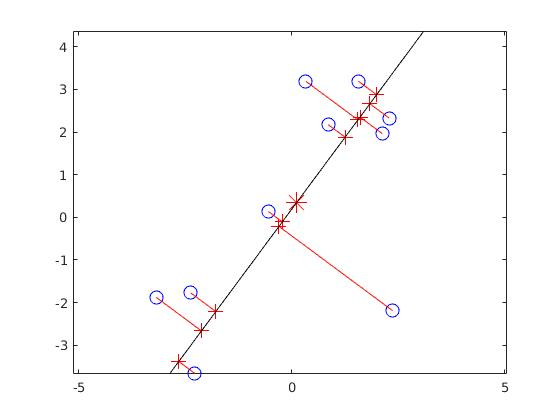
\includegraphics[width=0.8\linewidth]{./figs/pcaDemo.jpg}
% 
    \caption{Imagem retirada de \cite{machine-learning-book}. Exemplo de PCA com D = 2 e L = 1.}
    \label{fig:PCA}
\end{figure*}





\subsection{Conceitos de Probabilidade e Estatística}
\label{ssec:review-probabilidade}

Esta seção apresenta uma breve revisão de conceitos estatísticos necessários
para se entender a formulação na Seção \ref{ssec:tracking-parameter-fitting}.

\begin{itemize}

\item Variável Aleatória

Uma variável aleatória é uma variável cujos possíveis valores são resultados
numéricos de um fenômeno aleatório. Uma variável aleatória discreta é aquela
restrita a assumir valores dentre um conjunto contável de eventos. No texto que
segue, uma variável aleatória $\varkappa$ assume valores em um conjunto
$\Upsilon = \{\varphi_1, \varphi_2, \ldots\}$.

\item Probabilidade

Diz-se que a probabilidade da ocorrência de um evento é uma medida da confiança
que ele ocorra. A probabilidade é um número real entre 0 (indicando
impossibilidade) e 1 (indicando certeza). Quanto maior a probabilidade de um
evento, mais certeza há sobre sua ocorrência. No texto que segue, $\varkappa_1$
e $\varkappa_2$ são duas variáveis aleatórias, cada uma tomando valores em
$\Upsilon _1 = \{\varphi_1^1, \varphi_1^2, \ldots\}$ e $\Upsilon_2 =
\{\varphi_2^1, \varphi_2^2, \ldots\}$. Denota-se a probabilidade que
$\varkappa_1$ assuma valor $\varphi_1 \in \Upsilon_1$ como
$\mathpzc{p}(\varkappa_1 = \varphi_1)$ ou simplesmente $\mathpzc{p}(\varphi_1)$.

\item Probabilidade Conjunta

A probabilidade conjunta para $\varkappa_1$ e $\varkappa_2$ é a distribuição de
probabilidade que informa a probabilidade que $\varkappa_1 = \varphi_1$ e
$\varkappa_2 = \varphi_2$, $\forall (\varphi_1, \varphi_2) \in \Upsilon_1 \times
\Upsilon_2$, representada por $\mathpzc{p}(\varphi_1, \varphi_2)$. A definição
pode ser expandida para $k$ variáveis. Pode-se com isso definir a probabilidade
de um vetor discreto aleatório $k$-dimensional $\mathbf{\varkappa} =
[\varkappa_1, \ldots, \varkappa_k]$ como:

\begin{equation}
\mathpzc{p}(\mathbf{\varkappa}) = \mathpzc{p}(\varkappa_1, \varkappa_2, \ldots, \varkappa_k) 
\end{equation}

\item Probabilidade Condicional

Probabilidade condicional é a medida de probabilidade de um evento dado que um
outro evento ocorreu. A probabilidade condicional de $\varphi_1$ dado
$\varphi_2$ é escrita como $\mathpzc{p}(\varphi_1 | \varphi_2)$ e pode ser
calculada por:

\begin{equation}
\mathpzc{p}(\varphi_1 | \varphi_2) = \frac{\mathpzc{p}(\varphi_1, \varphi_2)}{\mathpzc{p}(\varphi_2)}
\end{equation}


\item Marginalização

Suponha que um dado processo estocástico seja governado por uma função de
probabilidade $\mathpzc{p}(\varphi_1,\varphi_2)$.  Suponha ainda que em dada
aplicação $\varphi_1$ seja uma variável de interesse e não se dê importância
para $\varphi_2$. Pode-se calcular a probabilidade $\mathpzc{p}(\varphi_1)$ ao
marginalizar-se $\varphi_2$:

\begin{equation}
\mathpzc{p}(\varphi_1) = \sum_{\varphi_2 \in \Upsilon_2} \mathpzc{p}(\varphi_1|\varphi_2)\mathpzc{p}(\varphi_2)
\end{equation}

\item Lei de Probabilidade Total

O seguinte resultado combina marginalização e probabilidade condicional:

\begin{equation}
\mathpzc{p}(\varphi_1|\varphi_3) = \sum_{\varphi_2 \in \Upsilon_2} \mathpzc{p}(\varphi_1|\varphi_2, \varphi_3)\mathpzc{p}(\varphi_2|\varphi_3)
\end{equation}

\item Distribuição Normal Multivariada

Uma função que comumente aparece em estatística é a distribuição normal. A
distribuição normal, ou gaussiana, em várias dimensões é escrita como:

\begin{equation}
\mathpzc{p}(\mathbf{\varphi}) = (2\pi)^{-\frac{k}{2}} | \mathbf{\Sigma} | ^ {-\frac{1}{2}} e^{-\frac{1}{2}(\mathbf{\varphi} - \mathbf{\mu})'\mathbf{\Sigma}^{-1}(\mathbf{\varphi} - \mathbf{\mu})}
\end{equation}

onde $\mathbf{\Sigma}$ é a matriz de co-variâncias e $\mathbf{\mu}$, um vetor
k-dimensional, é a média da distribuição. Quando uma variável k-dimensional
$\mathbf{\varkappa}$ possui distribuição de probabilidade dada por uma gaussiana
de média $\mathbf{\mu}$ e covariância $\mathbf{\Sigma}$, a seguinte notação é
utilizada:

\begin{equation}
\mathbf{\varkappa} \sim \mathcal{N}(\mathbf{\varkappa}; \mathbf{\mu}, \mathbf{\Sigma})
\end{equation}

A Figura \ref{fig:normal} mostra a forma de sino da Gaussiana bidimensional.

\begin{figure}[!htbp]
\centering
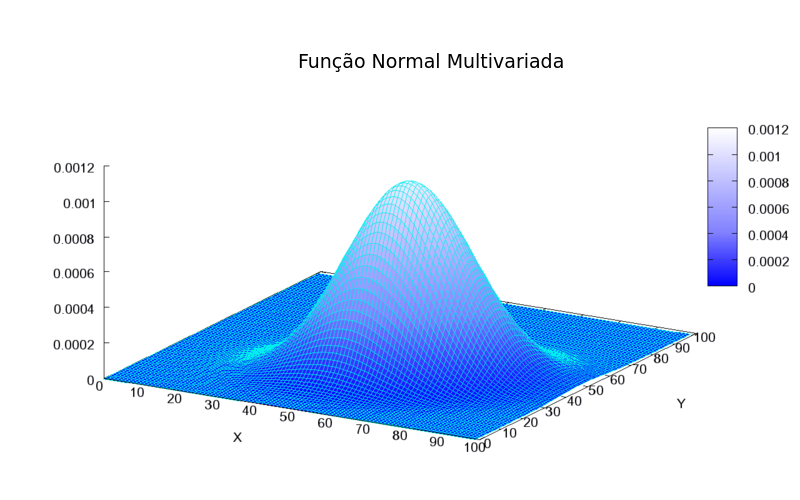
\includegraphics[width=0.7\textwidth]{figs/multivariate.png}
\caption{Distribuição Normal Bidimensional.}
%https://en.wikipedia.org/wiki/Multivariate_normal_distribution\
\label{fig:normal}
\end{figure}

\end{itemize}

\subsection{Formulação Estatística para o Ajuste de Parâmetros}
\label{ssec:tracking-parameter-fitting}

Como visto anteriormente, ajustar o PDM a uma imagem significa calcular o
conjunto $\mathbf{p} = \{s, \bm{R}, \bm{t}, \bm{q}\}$ que melhor ajusta o modelo
à imagem que se quer ajudar. Isso é feito minimizando-se a função custo

\begin{equation}
Q(\mathbf{p}) = R(\mathbf{p}) + \sum_{i=1}^n D_i(\mathbf{v}_i; \mathcal{I})
\label{eq:objective-function}
\end{equation}

na qual R é um fator de regularização que penaliza deformações complexas e $D_i$
denota uma medida de desalinhamento para o i-ésimo ponto de interesse na imagem
I \cite{facetracker}.

A Equação \ref{eq:objective-function} pode ser interpretada probabilisticamente
como a maximização da probabilidade dos parâmetros do modelo de forma que os
pontos de interesse estejam alinhados com suas respectivas localizações no
objeto em uma imagem \cite{facetracker}. A forma da função custo na Equação
\ref{eq:objective-function} assume implicitamente independência condicional
entre a detecção de cada ponto chave. Probabilisticamente falando, essa
independência condicional toma a forma:

\begin{equation}
\label{eq:conditional-independence}
\mathpzc{p}(\mathbf{p} | \{l_i = 1\}_{i=1}^n, \mathcal{I}) \varpropto \mathpzc{p}(\bf{p}) \prod_{i=1}^n \mathpzc{p}(l_i = 1 | \mathbf{v}_i, \mathcal{I})
\end{equation}

A variável discreta $l_i \in \{1, -1\}$ indica se o i-ésima ponto chave está
alinhado ou desalinhado, sendo $l_i=1$ no primeiro caso e $l_i=-1$ no segundo.
Na Equação \ref{eq:conditional-independence} o símbolo $\varpropto$ indica que
existe uma relação de proporção direta entre os termos a esquerda e a direita do
símbolo. Deixando mais claro, a notação $\mathpzc{a} \varpropto \mathpzc{b}$
significa que $\exists k \in \mathbb{R}$ tal que $\mathpzc{a} = k \mathpzc{b}$.
Como se está falando de probabilidade, vale notar que a constante deve ser
positiva e, portanto, maximizar o lado direito implica em maximizar o lado
esquerdo da Equação \ref{eq:conditional-independence}.  Para se obter a Equação
\ref{eq:objective-function}, aplica-se o logaritmo em ambos os lados da Equação
\ref{eq:conditional-independence} para transformar os produtos em somatório.
Além disso, algoritmos de otimização são comumente escritos para minimizar
funções e não para as maximizar. Por esse motivo, inverte-se o sinal da equação
obtida de forma que maximizar $f(\mathbf{x})$ é o mesmo que minimizar
$-f(\mathbf{x})$. Obtém-se então uma forma para as componentes de Q na Equação
\ref{eq:objective-function}:

\begin{equation}
\label{eq:P}
P(\mathbf{p}) = 
-\ln
(
\mathpzc{p}(\mathbf{p})
)
\end{equation}

\begin{equation}
D(\mathbf{v}_i; I) =
-\ln
(
\mathpzc{p}(l_i=1 | \mathbf{x}_1, \mathcal{I})
)
\end{equation}

Em \cite{facetracker}, utiliza-se a seguinte função para a probabilidade de alinhamento de uma localização $\bf{x}$ de um ponto chave: 

\begin{equation}
p(l_i = 1|\textbf{v},\mathcal{I}) = \frac{1}{1 + \exp{\{}l_iC_i(\textbf{v};\mathcal{I}){\}}}
\label{eq:alg1}
\end{equation}

Sendo $C_i$ o classificador que distingue locações alinhadas de desalinhadas
\cite{saragih2011deformable}. Ainda em \cite{facetracker}, o classificador $C_i$
utilizado é um de regressão logística aplicado em uma janela $\bf{\Omega_x}$ de
pixeis ao redor de $\bf{x}$.

Para completar a abordagem é preciso especificar $p(\bf{p})$ em \ref{eq:P}. Este
termo indica um conhecimento prévio sobre a distribuição dos parâmetros. Quando
se assume que todas as configurações são igualmente prováveis a formulação em
\ref{eq:conditional-independence} leva a uma estimação dos parâmetros \textbf{p}
por maximização de probabilidade, ou, em inglês, \textit{Maximum Likelihood}.
Quando, por outro lado, supõe-se uma distribuição não uniforme dos parâmetros,
tem-se uma estimação de Máximo a Priori (MAP) \cite{saragih2011deformable}.
Lembrando que para o MDP $\mathbf{p}=\{s,\mathbf{R},\mathbf{t},\mathbf{q}\}$,
$\mathpzc{p}(\mathbf{p})$ é especificado por partes. Em geral, assume-se um
modelo gaussiano para os parâmetros não rígidos $\mathbf{q}$ e uma probabilidade
uniforme sobre os parâmetros rígidos $\{s,\mathbf{R},\mathbf{t}\}$
\cite{facetracker}. O que leva a distribuição a priori:

\begin{equation}
\mathpzc{p}(\mathbf{p}) \varpropto \mathcal{N}(\mathbf{q}; 0, \mathbf{\Lambda})
\label{eq:Lambda}
\end{equation}

com $\mathbf{\Lambda} = \text{diag}\{[ \lambda_1; \ldots; \lambda_m]\}$, isto é,
a matriz diagonal contendo os autovalores dos modos de deformação aprendidos
pelo PCA. Nota-se que quanto maior o valor de $\lambda_i$ mais lentamente decai
a distribuição normal em \ref{eq:Lambda}. Colocando de outra forma, um maior
$\lambda_i$ indica que é mais provável uma componente $p_i$ em $\mathbf{p}$ de
alta magnitude.


\subsection{Otimização de Probabilidade por Deslocamento Regularizado de Média}

Devido ao erro de truncamento herdado do PCA, o modelo utilizado não pode
reconstruir perfeitamente a localização perfeita das poses chaves
\cite{saragih2011deformable}. O erro de truncamento é modelado nesta técnica
por:

\begin{align}
y_i = x_i + \epsilon_i
\label{eq:erro-trunc}
\end{align}

sendo $\epsilon_i \sim \mathcal{N}(\epsilon_i; 0, \rho I)$, $y_i$ a variável
aleatória representando a posição real da i-ésima pose chave e o parâmetro
$\rho$ pode ser aprendido durante o treinamento. A Equação \ref{eq:erro-trunc}
nos dá uma forma para $p(y_i | x_i)$:

\begin{equation}
p(y_i | v_i) = N(y_i; v_i, \rho I)
\end{equation}

Para a próxima etapa assume-se que existe um conjunto de candidatos $\Phi_i$
para cada marcador i do modelo. Por exemplo $\Phi_i$ pode denotar os pontos em
uma região de busca pelo i-ésimo ponto chave. Tratando a localização real dos
marcadores $y_i$ como uma variável escondida, pode-se marginalizá-la da
probabilidade de alinhamento dos marcadores:

\begin{equation}
p(l_i = 1|v_i, I) = \sum_{y_i \in \Phi_i} p(l_i = 1| y_i, \mathcal{I})p(y_i|v_i)
\end{equation}

O termo $p(l_i = 1| y_i, \mathcal{I})$ é renomeado $\pi_{y_i}$ e a equação é reescrita:

\begin{equation}
\label{eq:eq32}
p(l_i = 1|\mathbf{v}_i, \mathcal{I}) = \sum_{\mathbf{y}_i \in \mathbf{\Phi}_i} \pi_{\mathbf{y}_i} N(\mathbf{v}_i; \mathbf{y}_i, \rho \mathcal{I})
\end{equation}

Substituindo \ref{eq:eq32} em \ref{eq:conditional-independence}
 obtém-se:

\begin{equation}
p(p|\{l_i=1\}_{i=1}^n, \mathcal{I}) \varpropto p(p) \prod_{i=1}^n \sum_{\mathbf{y}_i \in \mathbf{\Phi}_i}
\pi_{y_i} N(\mathbf{v}_i; \mathbf{y}_i, \rho \mathbf{I})
\label{eq:eq23}
\end{equation}

A Equação \ref{eq:eq23} pode ser minimizada por um processo iterativo que
envolve calcular o vetor deslocamento de média $v = [v_1, v_2, \ldots, v_n]$ e a
atualização dos parâmetros $\Delta p$ através de:

\begin{equation}
\textbf{v}_i = \Bigg(\sum\limits_{\textbf{y}_i \in \Psi_i} \frac{\pi_{\textbf{y}_i}\mathcal{N}(\textbf{v}_i^c;\textbf{y}_i,\rho\textbf{I})}{\sum\nolimits_{\textbf{z}_i \in \Psi_i} \pi_{\textbf{z}_i}\mathcal{N}(\textbf{v}_i^c;\textbf{z}_i,\rho\textbf{I})
}\textbf{y}_i\Bigg) - \textbf{v}_i^c
\label{eq:alg3}
\end{equation}

e

\begin{equation}
\Delta\textbf{p} = -(\rho\tilde{\mathbf{\Lambda}}^{-1} + \textbf{J}^T\textbf{J})^{-1}(\rho\tilde{\mathbf{\Lambda}}^{-1}\textbf{p} - \textbf{J}^T\textbf{v})
\label{eq:alg4}
\end{equation}

onde $\tilde{\mathbf{\Lambda}}$ é a matriz diagonal cujos elementos da diagonal
são os elementos do vetor $[\mathbf{0}, \lambda_1, \ldots, \lambda_m]$,
$\mathbf{J} = [\mathbf{J}_1; \ldots; \mathbf{J}_n]$ é o jacobiano do PDM(ver
Equação \ref{eq:PDM-equation}) e $\mathbf{x}_c^i$ é a estimação atual do
$i$-ésimo marcador.




               
\section{Estimação de Profundidade}

Um problema que aparece quando se trata de visão monocular é a falta de
informação de profundidade, uma vez que o processo de formação de uma imagem
consiste na captura apenas de duas das três dimensões espaciais. Com isso, uma
infinidade de objetos tridimensionais podem ser relacionados a uma mesma imagem
bidimensional. Ou seja, uma imagem não contém informações suficientes para
reconstruir uma cena tridimensional \cite{bolles1987epipolar}. No entanto, uma
aplicação que necessite de informação de tridimensionalidade a partir de captura
de imagens pode utilizar duas ou mais câmeras cujos parâmetros intrínsecos são
conhecidos.

\subsection{Modelo da Câmera}

Nesta seção é definido o modelo de câmera necessário para a extração dos
parâmetros intrínsecos utilizados neste trabalho. 

Primeiramente, apresenta-se o modelo de projeção dos pontos do sistema de
coordenadas do mundo para o plano da imagem. Considera-se que o centro da
projeção é a origem do sistema de coordenadas e que $\{(X,Y,Z), Z = f\}$
corresponde ao plano da imagem. Usando um modelo de câmera \textit{pinhole}, um
ponto no sistema de coordenadas do mundo $\mathcal{X} = (X,Y,Z)^T$ é mapeado
para um ponto no plano da imagem como mostrado na Figura \ref{fig:projeção}.

\begin{figure}[h!]
\centering
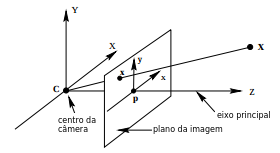
\includegraphics[width=.5\linewidth]{figs/TG_pinhole_1_pt.png}
\caption{Projeção de um ponto no mundo para o plano da imagem (adaptado de \cite{hartley2003multiple}).}
\label{fig:projeção}
\end{figure}

Por aplicação de uma semelhança de triângulos ilustrada na Figura \ref{fig:mapeamento} é possível mostrar que o ponto $(X,Y,Z)^T$ do espaço é mapeado para o ponto $(fX/Z,fY/Z,f)^T$ no domínio da imagem, ou seja:

\begin{equation}
(X,Y,Z)^T \mapsto (fX/Z,fY/Z)^T
\label{eq:3d_mapPonto}
\end{equation}


\begin{figure}[h!]
\centering
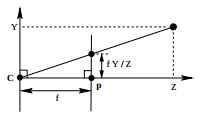
\includegraphics[width=.5\linewidth]{figs/TG_pinhole_2.png}
\caption{Mapeamento de um ponto no mundo para o plano da imagem (retirado de \cite{hartley2003multiple}).}
\label{fig:mapeamento}
\end{figure}

Sendo os pontos no mundo e na imagem representados por vetores homogêneos, então
a projeção central é expressa como um mapeamento linear de suas coordenadas
homogêneas:

\begin{align}
\left(\begin{array}{c}
X\\
Y\\
Z\\
1
\end{array}\right) \mapsto
\left(\begin{array}{c}
fX\\
fY\\
Z
\end{array}\right) =
\left[\begin{array}{cccc}
f & 0 & 0 & 0\\
0 & f & 0 & 0\\
0 & 0 & 1 & 0
\end{array}\right]
\left(\begin{array}{c}
X\\
Y\\
Z\\
1
\end{array}\right)
\label{eq:3d_vetHomogeneo1}
\end{align}

Fazendo $\mathcal{X}$ o vetor homogêneo $(X,Y,Z,1)^T$ e $\mathtt{x}$ o ponto na
imagem representado por um vetor de 3 dimensões, tem se que $\bm{\mathcal{P}}$
representa a matriz de projeção da câmera, sendo que a relação entre esses
termos dada por:

\begin{equation}
\mathtt{x} = \bm{\mathcal{P}}\mathcal{X}
\label{eq:3d_Pmatriz}
\end{equation}

Este mapeamento assume que a origem do sistema de coordenadas no plano da imagem
é a mesma do sistema de coordenadas da câmera; porém, isso nem sempre é verdade
\cite{hartley2003multiple}. Na prática tem-se que:

\begin{equation}
(X,Y,Z)^T \mapsto (fX/Z + p_x,fY/Z + p_y)^T
\label{eq:3d_mapForaCentro}
\end{equation}


sendo $p_x$ e $p_y$ são as coordenadas do \textbf{ponto principal}. Desta forma,
ao expressar em coordenadas homogêneas a equação é:

\begin{align}
\left(\begin{array}{c}
X\\
Y\\
Z\\
1
\end{array}\right) \mapsto
\left(\begin{array}{c}
fX + Zp_x\\
fY + Zp_y\\
Z
\end{array}\right) =
\left[\begin{array}{cccc}
f & 0 & p_x & 0\\
0 & f & p_y & 0\\
0 & 0 & 1 & 0
\end{array}\right]
\left(\begin{array}{c}
X\\
Y\\
Z\\
1
\end{array}\right)
\label{eq:3d_vetHomogeneo2}
\end{align}

Definindo $\bf{K}$ como:

\begin{align}
\bf{K} =
\left[\begin{array}{ccc}
f & 0 & p_x\\
0 & f & p_y\\
0 & 0 & 1
\end{array}\right]
\label{eq:3d_matIntrinseca}
\end{align}

tem-se que $\mathtt{x}$ é dado por:

\begin{equation}
\mathtt{x} = \bf{K}[\bf{I}|0]\mathcal{X}
\label{3d_camModel1}
\end{equation}

A matriz $\bf{K}$ é chamada de matriz intrínseca da câmera.

No geral, pontos no mundo serão expressados como termos de diferentes sistemas
de coordenadas. Isso implica que a origem do sistema de coordenadas do mundo
geralmente não coincide com a origem do sistema de coordenadas da câmera
\cite{hartley2003multiple}, esses dois sistemas de coordenadas são então
relacionados por rotação e translação, como visto na Figura \ref{fig:trans_rot}
.

\begin{figure}[h!]
\centering
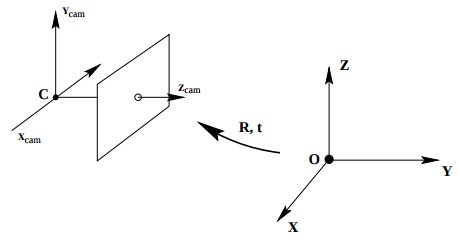
\includegraphics[width=.5\linewidth]{figs/TG_rot_tr.png}
\caption{Transformação entre as coordenadas globais e as coordenadas da câmera por rotação e translação (retirado de \cite{hartley2003multiple}).}
\label{fig:trans_rot}
\end{figure}

Se $\tilde{\mathcal{X}}$ é um vetor não homogêneo que representa um ponto no
sistema de coordenadas do mundo e $\tilde{\mathcal{X}}_{cam}$ representa o mesmo
ponto no sistema de coordenadas da câmera, então pode se dizer que
$\tilde{\mathcal{X}}_{cam} = \bf{R}(\tilde{\mathcal{X}} - \tilde{C})$, onde
$\tilde{C}$ representa o centro da câmera no sistema de coordenadas do mundo e
$\bf{R}$ é a matriz de rotação que representa a orientação do sistema de
coordenadas da câmera. A equação em termos de coordenadas homogêneas pode ser
descrita por:

\begin{align}
\mathcal{X}_{cam} =
\left[\begin{array}{cc}
\bf{R} &  -\bf{R}\tilde{C}\\
0 & 1
\end{array}\right]
\mathcal{X}
\label{eq:3d_matRot}
\end{align}

na qual $\mathtt{x}$ é descrito por:

\begin{equation}
\mathtt{x} = \bf{K}\bf{R}[\bf{I}|-\tilde{C}]\mathcal{X}
\label{eq:3d_camModel2}
\end{equation}

Usando a matriz de projeção da câmera definida na Equação \ref{eq:3d_Pmatriz},
$\bm{\mathcal{P}}$ pode ser escrito como:

\begin{equation}
\bm{\mathcal{P}} = \bf{K}\bf{R}[\bf{I}|-\tilde{C}]
\label{eq:3d_PModel1}
\end{equation}


Este é o modelo básico dado por uma câmera do tipo \textit{pinhole}. É muitas
vezes conveniente não explicitar o centro da câmera \cite{hartley2003multiple},
mas representar a transformação de um ponto no mundo para um ponto na imagem
como $\tilde{\mathcal{X}}_{cam} = \bf{R}\tilde{\mathcal{X}} + \bf{t}$, sendo
$\bf{t} =-\bf{R}\tilde{C}$. Neste caso, a matriz dos parâmetros intrínsecos da
câmera $\bm{\mathcal{P}}$  é escrita como

\begin{equation}
\bm{\mathcal{P}} = \bf{K}[\bf{R}|\bf{t}]
\label{eq:3d_PModel2}
\end{equation}

\subsection{Triangulação}

Para a reconstrução tridimensional da cena, deve se resolver o problema da
triangulação. Supondo que um ponto $\mathcal{X}$ em $R^3$ é visível em duas
imagens e que as distâncias focais $f_1$ e $f_2$ correspondentes a essas duas
imagens são conhecidas, sendo $u$ e $u'$ as projeções do ponto $\mathcal{X}$ nas
imagens, as linhas no espaço correspondentes aos dois pontos da imagem podem
ser, a partir desses dados, facilmente computadas. O problema da triangulação é
achar a interseção destas duas linhas no espaço \cite{hartley1997triangulation}.
Este modelo pode ser visualizado na Figura \ref{fig:disp_cameras}.

\begin{figure}[h!]
\centering
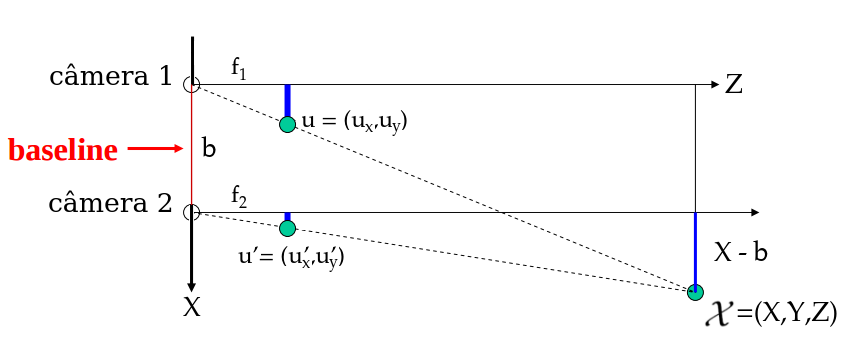
\includegraphics[width=.72\linewidth]{figs/TG_triangulation_pdf_washington_pt2.png}
\caption{Disposição das câmeras (adaptado de \cite{stereovision-washington-pdf}).}
\label{fig:disp_cameras}
\end{figure}

%https://courses.cs.washington.edu/courses/cse455/09wi/Lects/lect16.pdf

Com a Figura \ref{fig:disp_cameras} como referência, é possível, por semelhança
de triângulos, derivar as seguintes equações para o valor $X$ do ponto no
sistema de coordenadas do mundo.

\begin{equation}
X = (u_x/f_1)  Z
\label{eq:3d_realX1}
\end{equation}   

ou

\begin{equation}
X = (u'_x/f_2)  Z + b
\label{eq:3d_realX2}
\end{equation}  

A relação do valor $Y$ do ponto no sistema de coordenadas do mundo pode também
ser relacionado com sua projeção no plano da imagem por uma semelhança de
triângulos, como mostrado na Figura \ref{fig:mapeamento}. As equações de $Y$ são
mostradas a seguir.

\begin{equation}
Y = (u_y/f_1) Z
\label{eq:3d_realY1}
\end{equation}      

ou

\begin{equation}
Y = (u'_y/f_2) Z
\label{eq:3d_realY2}
\end{equation}  


A partir das Equações \ref{eq:3d_realX1} e \ref{eq:3d_realX2} é possível
expressar o valor da profundidade $Z$ do ponto como

\begin{equation}
Z = f_1  f_2  b / (u_x  f_2 - u'_x  f_1)
\label{eq:3d_Zequation}
\end{equation}


Em que $b$ se refere a \textit{baseline}, ou seja, a distância fixa entre as
câmeras, $u'_x$ e $u_x$ são os valores em $x$ da projeção do ponto no plano da
imagem das câmeras 1 e 2, respectivamente, e $f_1$ e $f_2$ são as distâncias
focais obtidas a partir da matriz intrínseca de cada câmera, esta que pode ser
derivada através da matriz da câmera, também chamada de matriz de calibração. A
matriz de calibração pode ser obtida usando a \textit{Calibration Toolbox for
Matlab}, onde a partir de uma série de imagens de um tabuleiro de xadrez
(\textit{chessboard}) capturadas pela mesma câmera é possível relacionar pontos
iguais em várias imagens e então derivar a matriz de calibração
\cite{bouguetML}.

\section{Renderização de Objetos Tridimensionais}

A renderização de objetos tridimensionais neste trabalho foi feita utilizando a
\nomenclature{API}{\textit{Application program interface}} Interface de
Programação de Aplicações (API) \nomenclature{OpenGL}{\textit{Open Graphics
Library}} \textit{Open Graphics Library} (OpenGL). Para a compreensão de como
esta renderização é feita, deve-se entender como é formado um objeto e como ele
é posicionado no sistema de coordenadas. 

Um triângulo é a estrutura mais básica em computação tridimensional
\cite{openGlWikibooks} e todos os objetos neste trabalho são representados
computacionalmente por um conjunto de pequenos triângulos texturizados. Um
triângulo é definido por três vértices e cada vértice é composto por três
coordenadas: $X_p$, $Y_p$ e $Z_p$.
% [wikibooks.org/wiki/OpenGL_Programming/Modern_OpenGL_Introduction]

A informação de um objeto tridimensional completamente renderizado é armazenada
em um \nomenclature{VAO}{\textit{Vertex Array Object}} \textit{Vertex Array
Object} (VAO), uma estrutura que contém um ou mais
\nomenclature{VBO}{\textit{Vertex Buffer Object}} \textit{Vertex Buffer Objects}
(VBOs). Um VBO é um \textit{buffer} de memória contido na memória de alta
velocidade da placa de vídeo, e contém informações sobre os vértices
\cite{openGlOrg}. Podem, por exemplo, conter as coordenadas dos vértices ou
talvez a cor associada a cada vértice.

% [opengl.org/wiki/Tutorial2:_VAOs,_VBOs,_Vertex_and_Fragment_Shaders_(C_/_SDL)]

Desta maneira é possível criar a forma de um objeto construindo um VBO que
contém as coordenadas de todos os triângulos que compõem o objeto; porém, assim
sempre existirão duplicatas quando vértices de dois triângulos compartilharem
uma aresta \cite{openGlTutorial}. Para evitar esta replicação desnecessária, os
pontos em si são guardados separadamente do objeto e a malha é construída com
índices para estes pontos. O efeito desta indexação é ilustrado na Figura
\ref{fig:VBO}.

\begin{figure}[h!]
\centering
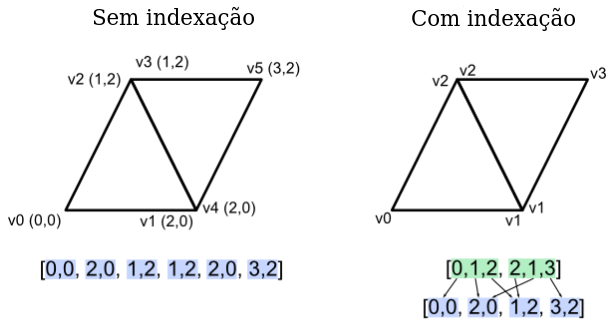
\includegraphics[width=.5\linewidth]{figs/TG_VBO_index_pt.png}
\caption{Indexação do VBO (adaptado de \cite{openGlTutorial}).}
\label{fig:VBO}
\end{figure}

Além disso, esta forma de representação tem a  vantagem de apresentar uma
estrutura bem semelhante a forma como a geometria tridimensional  é armazenada
em um arquivo no formato OBJ. Esta semelhança faz com que o carregamento destes
arquivos para a renderização utilizando OpenGL fique bem mais simples.

Para definir um objeto completamente e não apenas sua forma, se faz necessário o
uso de outros VBOs como, por exemplo, um VBO contendo informações das
coordenadas de textura e um VBO contendo informações das direções normais a
superfície de cada triângulo. A direção normal é importante para que se aplique
iluminação sobre o objeto renderizado e sem iluminação adequada não seria
possível ver os detalhes da superfície, apenas seu contorno.

% [opengl-tutorial.org/intermediate-tutorials/tutorial-9-vbo-indexing/]

Para o posicionamento do objeto no sistema de coordenadas ser definido,
primeiramente são definidas as seguintes matrizes de transformação: translação,
rotação e escala.

A matriz de translação é dada por:

\begin{align}
\left[\begin{array}{cccc}
1 & 0 & 0 & D_y\\
0 & 1 & 0 & D_x\\
0 & 0 & 1 & D_z\\
0 & 0 & 0 & 1
\end{array}\right]
\left(\begin{array}{c}
X_p\\
Y_p\\
Z_p\\
1
\end{array}\right) =
\left(\begin{array}{c}
X_p + D_x\\
Y_p + D_y\\
Z_p + D_z\\
1
\end{array}\right)
\label{eq:rend_translationMat}
\end{align}

A matriz de escala por:

\begin{align}
\left[\begin{array}{cccc}
S_x & 0 & 0 & 0\\
0 & S_y & 0 & 0\\
0 & 0 & S_z & 0\\
0 & 0 & 0 & 1
\end{array}\right]
\left(\begin{array}{c}
X_p\\
Y_p\\
Z_p\\
1
\end{array}\right) =
\left(\begin{array}{c}
S_x \cdot X_p\\
S_y \cdot Y_p\\
S_z \cdot Z_p\\
1
\end{array}\right)
\label{eq:rend_scaleMat}
\end{align}

E as matrizes de rotação:

Rotação no eixo X:

\begin{align}
\left[\begin{array}{cccc}
1 & 0 & 0 & 0\\
0 & cos\theta & -sen\theta & 0\\
0 & sen\theta & cos\theta & 0\\
0 & 0 & 0 & 1
\end{array}\right]
\left(\begin{array}{c}
X_p\\
Y_p\\
Z_p\\
1
\end{array}\right) =
\left(\begin{array}{c}
X_p\\
cos\theta \cdot Y_p - sen\theta \cdot Z_p\\
sen\theta \cdot Y_p + cos\theta \cdot Z_p\\
1
\end{array}\right)
\label{eq:rend_rotationMatX}
\end{align}

Rotação no eixo Y:

\begin{align}
\left[\begin{array}{cccc}
cos\theta & 0 & sen\theta & 0\\
0 & 1 & 0 & 0\\
-sen\theta & 0 & cos\theta & 0\\
0 & 0 & 0 & 1
\end{array}\right]
\left(\begin{array}{c}
X_p\\
Y_p\\
Z_p\\
1
\end{array}\right) =
\left(\begin{array}{c}
cos\theta \cdot X_p + sen\theta \cdot Z_p\\
Y_p\\
-sen\theta \cdot X_p + cos\theta \cdot Z_p\\
1
\end{array}\right)
\label{eq:rend_rotationMatY}
\end{align}

Rotação no eixo Z:

\begin{align}
\left[\begin{array}{cccc}
cos\theta & -sen\theta & 0 & 0\\
sen\theta & cos\theta & 0 & 0\\
0 & 0 & 1 & 0\\
0 & 0 & 0 & 1
\end{array}\right]
\left(\begin{array}{c}
X_p\\
Y_p\\
Z_p\\
1
\end{array}\right) =
\left(\begin{array}{c}
cos\theta \cdot X_p - sen\theta \cdot Y_p\\
sen\theta \cdot X_p + cos\theta \cdot Y_p\\
Z_p\\
1
\end{array}\right)
\label{eq:rend_rotationMatZ}
\end{align}

% [//open.gl/transformations]

Os vértices são aqui definidos como vetores de quatro dimensões pois em OpenGL
este quarto parâmetro, chamado de $W_p$, define se o vetor é uma posição no
espaço, caso $W_p = 1$, ou se o vetor é uma direção, caso $W_p = 0$.

Com essas matrizes definidas pode-se derivar outras três matrizes: a matriz do
modelo, a matriz de visualização e a matriz de projeção. Essas matrizes são
úteis para separar as transformações de forma eficiente.

Um objeto é definido por um conjunto de vértices e as coordenadas $X_p$, $Y_p$ e
$Z_p$ destes vértices são definidos relativamente ao centro do objeto, ou seja,
se um vértice está localizado em $(0,0,0)$, então ele está localizado no centro
do objeto \cite{openGlTutorial}. Para mover o objeto no espaço virtual
utiliza-se a matriz do modelo, que é um produto das matrizes de translação,
rotação e escala aplicadas no objeto. A aplicação desta transformação  coloca
vértices do objeto no sistema de coordenadas do espaço. A Figura
\ref{fig:mat_modelo} ilustra a transformação.

\begin{figure}[h!]
\centering
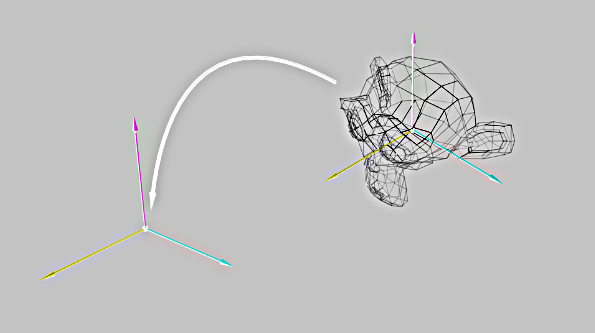
\includegraphics[width=.5\linewidth]{figs/TG_model_matrix_neg.png}
\caption{Efeito da Matriz do Modelo (adaptado de \cite{openGlTutorial}).}
\label{fig:mat_modelo}
\end{figure}

% [opengl-tutorial.org/beginners-tutorials/tutorial-3-matrices/]

A matriz de visualização pode ser interpretada como o posicionamento e angulação
de uma câmera que irá apontar para o cenário observado, de forma que é possível
mover esta câmera para observar o objeto a partir de outras posições e direções
arbitrárias. Apesar da interpretação acima, o  que realmente acontece é que não
é a câmera que move e sim todo o cenário, incluindo o objeto. A aplicação desta
transformação por meio do produto a esquerda com a matriz de visualização coloca
as coordenadas dos vértices no sistema de coordenadas da câmera. A Figura
\ref{fig:mat_visao} ilustra o que acontece.

\begin{figure}[h!]
\centering
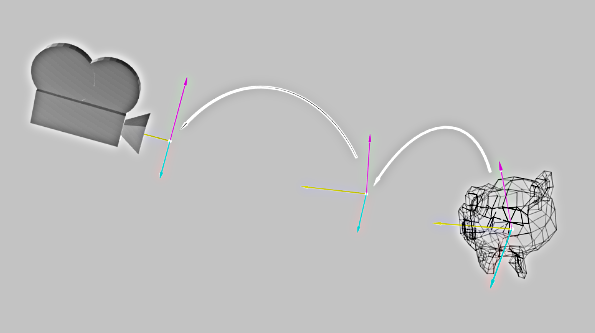
\includegraphics[width=.5\linewidth]{figs/TG_view_matrix_neg.png}
\caption{Efeito da Matriz de Visualização (adaptado de \cite{openGlTutorial}).}
\label{fig:mat_visao}
\end{figure}

A função da matriz de projeção é basicamente fazer com que objetos mais
distantes da câmera pareçam menores, como ocorre no mundo real. No sistema de
coordenadas da câmera dois vértices com um mesmo par de coordenadas $(X_p,Y_p)$
serão renderizados no mesmo local, o que não é sempre verdade. Isto acontece
pois a coordenada $Z_p$ não está sendo levada em conta. Para a profundidade ser
levada em conta e a perspectiva corrigida a matriz de projeção transforma o
espaço de visão da câmera, que inicialmente é um hexaedro irregular, em um cubo
\cite{openGlTutorial}, com isso os objetos são deformados de modo que o que está
mais próximo da câmera pareça maior e o que está mais distante da câmera pareça
menor, tendo-se, por fim, um sistema de coordenadas homogêneas. As Figura
\ref{fig:mat_proj} ilustra o que acontece.

\begin{figure*}[!htb]
   \centering
\begin{tabular}{cc}
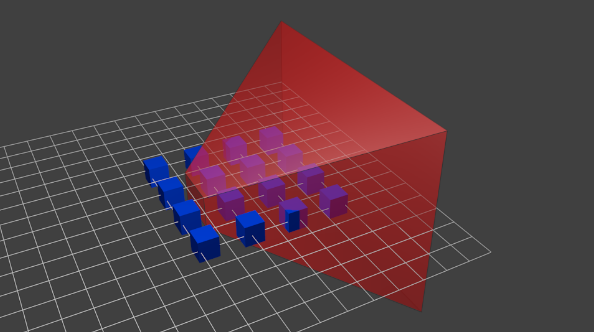
\includegraphics[width=0.4\linewidth]{./figs/TG_projection_matrix_1.png}&
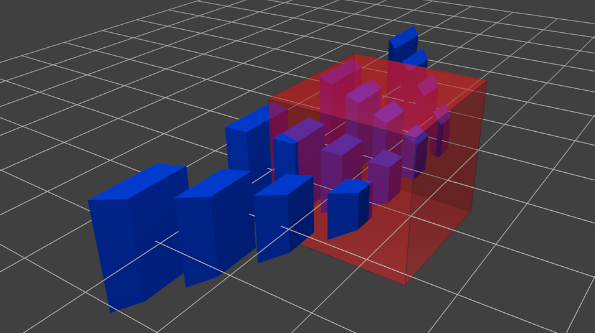
\includegraphics[width=0.4\linewidth]{./figs/TG_projection_matrix_2.png}
\end{tabular}
    \caption{Efeito da Matriz de Projeção (retirado de \cite{openGlTutorial})}
    \label{fig:mat_proj}
\end{figure*}

Um diagrama do efeito dessas três matrizes no sistemas de coordenadas onde se
encontra o objeto pode ser visualizado na Figura \ref{fig:mat_diagrama}.

\begin{figure}[h!]
\centering
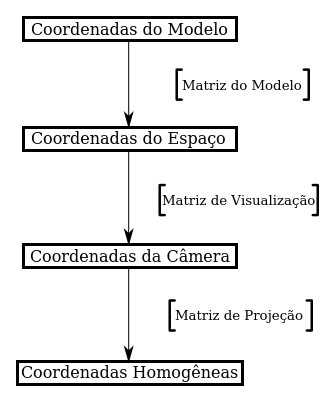
\includegraphics[width=.45\linewidth]{figs/TG_matrices_diagram_pt.png}
\caption{Diagrama do efeito das matrizes (adaptado de \cite{openGlTutorial}).}
\label{fig:mat_diagrama}
\end{figure}

\section{Mistura de Poses}

  Mesmo nas mais simples animações comerciais, um modelo tridimensional
utilizado costuma ser composto por milhares de vértices e polígonos.
Renderizar um rosto expressivo requer definir valores para cada um dos
vértices envolvidos. Adicione ao problema o fato de que um vídeo de poucos
segundos pode exigir centenas de expressões ligeiramente diferente uma da
outra para que o animação seja percebida de forma suave.
    
  Uma das técnicas utilizadas pelos animadores digitais é a Animação
Esqueletal (\textit{Skeletal Animation}) na qual se define um esqueleto
sobre o modelo tridimensional, de forma que movimento de cada ponto sobre o
modelo está atrelado ao movimento de rotação e translação das juntas. O
artista pode então posicionar as juntas em poses chaves do movimento e pedir
para que o computador interpole os pontos intermediários. Comumente, mesmo
depois da interpolação é necessário que o artista retoque manualmente alguns
pontos para que o resultado se torne ainda mais atrativo.
    
    A Figura \ref{fig:rigged-models}, retirada do tutorial em \cite{rigs-tutorial}, mostra a tela do problema \textit{Blender} enquanto o usuário define os \textit{ossos} ou a \textit{armadura} sobre o modelo. Mais tarde, pode-se movimentar os ossos individualmente e a malha do modelo se moverá juntamente.
    
    
\begin{figure*}[!htb]
   \centering
\begin{tabular}{cc}
  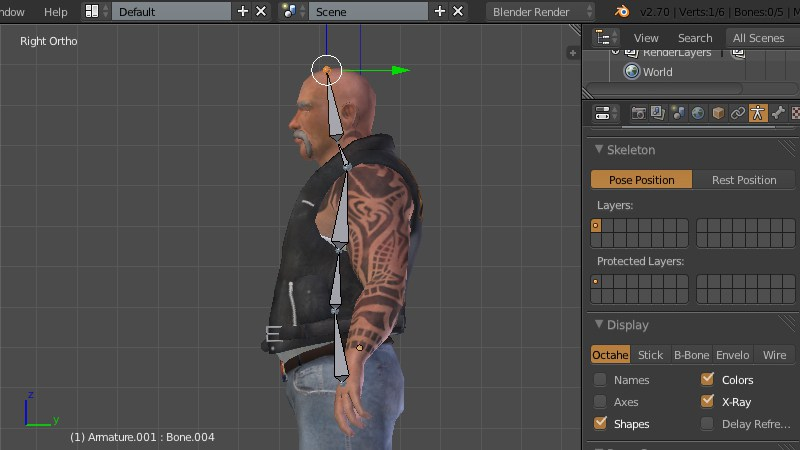
\includegraphics[width=0.4\linewidth]{./figs/blender_armature_image.jpg}
  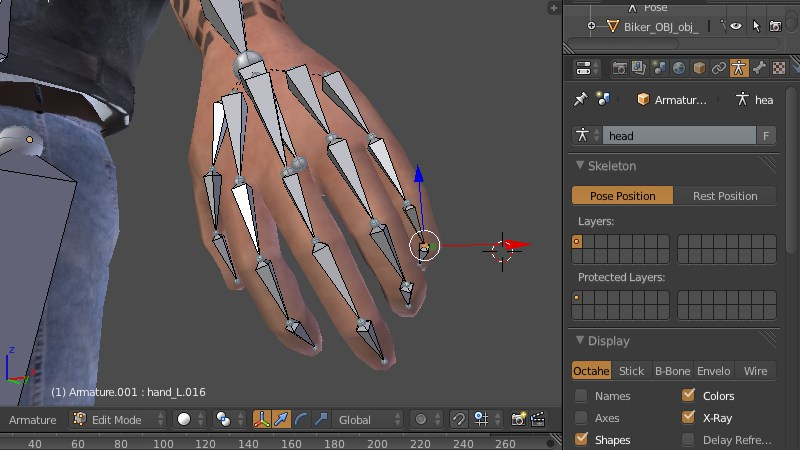
\includegraphics[width=0.4\linewidth]{./figs/blender_armature_image_14.jpg}
\end{tabular}

  \caption{ Tela do programa gratuito de código aberto \textit{Blender} (retirado de \cite{rigs-tutorial}). Cada um dos elementos em cinza é um osso do modelo. O termo utilizado no meio artístico é que se trata de um modelo \textit{rigado}.}

\label{fig:rigged-models} 
\end{figure*}
    
  O uso de \textit{rigged models} é recomendado para animar cenas onde o corpo
inteiro do personagem se mexe. No entanto, é ineficiente para animar
expressões faciais. O problema é que as transformações permitidas pelo modelo
de juntas se limita a transformações rígidas e a forma como os músculos do
rosto se comportam é melhor representada por transformações não rígidas, isto
é, deformações na geometria do corpo.
    
    A técnica de \nomenclature{MP}{\textit{Mistura de Poses}} Mistura de Poses -
MP, do inglês \textit{Blend Shapes} ou \textit{Morph Target}, é uma das
opções comumente empregadas para animar objetos deformáveis como a face
humana. Outros objetos comumente animados com essa técnica são peças de
roupa e pele, uma vez que esses objetos são dificilmente modelados por um
modelo esqueletal \cite{master-thesis-on-blend-shapes}. A técnica consiste
em gerar poses intermediárias como uma combinação linear de poses
pré-definidas. A Figura \ref{fig:blend-shapes-example-input} mostra três
poses utilizadas para a MP mostrada na Figura
\ref{fig:blend-shapes-example-output}.
    
    Em sua versão mais simples, a MP requer que cada um dos modelos
representando as poses chaves tenham a mesma quantidade de vértices. Mais do
que isso, é necessário que se seja capaz de mapear todos os pontos de um
modelo nos pontos de outro. Colocando de outra forma, dá-se um identificador
para cada vértice que compõe a malha do modelo
\cite{tutorial-supremo-on-blend-shapes}.    
    
\FloatBarrier
\begin{figure*}[!htb]
   \centering
  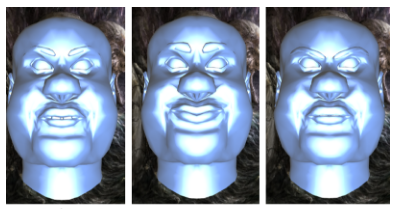
\includegraphics[width=0.7\linewidth]{./figs/inputToBlendShapes.png}

\caption{Três modelos a serem misturados pela técnica de \textit{Blend Shapes}
(retirado de \cite{tutorial-supremo-on-blend-shapes}). Respectivamente da
esquerda para a direita, os modelos representam a pose neutra, a expressão de
felicidade e de raiva. Nota-se a diferença na forma dos lábios e nas sobrancelhas.}

\label{fig:blend-shapes-example-input} 
\end{figure*}

\begin{figure*}[!htb]
   \centering
  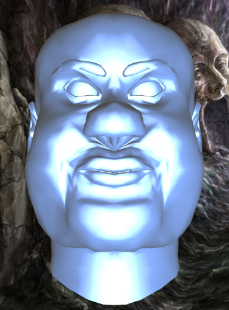
\includegraphics[width=0.6\linewidth]{./figs/outputOfBlendShapes.png}

\caption{Resultado obtido ao combinar 0.5 da pose alegre, 0.3 da pose com raiva e 0.2 da pose neutra (retirado de \cite{tutorial-supremo-on-blend-shapes}).}

\label{fig:blend-shapes-example-output} 
\end{figure*}

% \FloatBarrier
    
    Um modelo M(t) que se deforma no tempo é dado pela tupla de $N$ pontos
    tridimensionais $ ( v_1(t), v_2(t), \ldots,  v_N(t))$. Considere o espaço de
    poses ao longo do tempo $\Omega = \{ M(t), t \in R\}$  e amostre $L$ poses
    distintas $M_i = M(t_i), i = 1 \ldots L$. A MP consiste em construir o
    espaço das poses que podem ser obtidas como uma combinação linear das poses
    amostradas, limitado a fato de que a soma dos coeficientes da combinação
    seja unitária. Além disso, é comum que se defina uma das amostras como a
    pose neutra $M_1$. O peso dessa amostra neutra é escolhido como o negativo
    da soma das outras amostras mais um.
    
    Uma pose $J$ pertencente ao espaço de poses criado deve ser obtido por:    

\begin{equation}
    	J = \sum_{i=1}^L  w_i M_i
        \label{eq:J-mistura}
\end{equation}

Um pouco de manipulação pode deixar mais clara a forma como a mistura de
deformações não rígidas acontece.

\begin{equation}
    	J = w_1 M_1 + w_2 M_2 + \ldots + w_L M_L
\end{equation}

\begin{equation}
    	J = (1-(w_2 + w_3 + \ldots w_L)) M_1 + w_2 M_2 + \ldots + M_\theta + \ldots + w_L M_L
\end{equation}

\begin{equation}
    	J = M_1 + w_1(M_2 - M_1) + \ldots + w_L (M_L - M_1)
\end{equation}

\begin{equation}
    	J = M_1 + \sum_{i = 2}^L w_i \Delta M_i
        \label{eq:blendshapes}
\end{equation}

sendo $\Delta M_i = M_i - M_1$ é a deformação relativa entre $M_i$ e $M_1$. A
última equação deixa claro que as poses obtidas podem ser vistas como a soma de
deformações conhecidas superpostas com a pose neutra. 

Programas de animação utilizam a Equação \ref{eq:blendshapes} da seguinte
maneira: \begin{itemize}

  \item modela-se a pose neutra do seu personagem; 

    \item geram-se expressões chaves a partir da pose neutra apenas pela
      movimentação dos seus vértices;

    \item carrega-se a pose neutra e as demais no framework de mistura de poses
      chaves;

    \item mexendo-se em cursores associados ao peso de cada pose na mistura
      produzem-se  poses intermediárias que são marcadas a pontos no tempo do
      vídeo;

    \item pede-se então que o programa interpole as posições marcadas para que o
      resultado seja suave.

\end{itemize}

A técnica de Animação Esqueletal e a MP são semelhantes no fato em que o artista
configura poses chaves e então o computador completa as lacunas por meio de
interpolação. No entanto, as técnicas produzem resultados de natureza diferente.
Enquanto a primeira pode produzir um braço que tem a junta do cotovelo em
$45^\circ$, a MP produz um rosto que está meio bravo, meio alegre.

Colocando-se em termos bem simples, depois que os modelos para as poses chaves
estão prontos, a técnica de MP recebe um vetor de pesos e produz uma nova pose
como uma média ponderada das poses chaves.

  Programas que realizam a técnica de mistura de poses chaves não são novidade.
  O nosso objetivo é substituir a mão do artista mexendo os cursores de uma
  interface gráfica, por um programa que associa posições do cursor a
  propriedades do vídeo em execução.


\section{Estabilização do movimento}

Devido a ruídos oriundos do processo de captura de imagem e mesmo a
características estatísticas de alguns algoritmos de rastreamento, é comum que o
resultado da detecção oscile em torno do valor correto, mesmo quando a detecção
é feita adequadamente. Em muitas aplicações é desejável que se suavize o
resultado da detecção antes que este seja utilizado para a tomada de decisões. É
com esse objetivo que são utilizadas técnicas de filtragem digital. 

\subsection{Sequências e Sistemas Lineares Invariantes ao Deslocamento}
 
Para a discussão que segue, é dito que uma sequência é uma função $N_0
\rightarrow R$. Isto é, para cada número $n\in \{0,1,2,,\cdots\}$ a sequência
$\chi$ associa o número $\chi(n) \in R$.

Alguns sistemas podem ser descritos por meio de suas respostas a sequências de
entrada. Por exemplo, o sistema $H$  produz a sequência de saída $h(n)$ quando é
submetido a sequência de entrada $\chi(n)$.

Um sistema é dito linear quando vale a seguinte relação:

\begin{equation}
\gamma(n)_{\alpha \chi_1 + \beta \chi_2} = \alpha \gamma_{\chi_1}(n) + \beta \gamma_{\chi_2}(n)
\end{equation}

na qual $\gamma(n)_{\alpha \chi_1 + \beta \chi_2}$ é a resposta do sistema
quando submetido à sequência de entrada $\alpha \chi_1(n) + \beta \chi_2(n)$ e
$\gamma_{\chi_1}(n)$ e $\gamma_{\chi_2}(n)$ são as saídas do sistema quando
submetido a sequências de entrada $\chi_1(n)$ e $\chi_2(x)$ respectivamente. Em
palavras, o sistema é linear quando a sua resposta à combinação linear de dois
sinais é igual à combinação das suas respostas aos dois sinais quando aplicados
independentemente. 

Um sistema é invariante ao deslocamento quando:

\begin{equation}
\gamma_{\chi(n-k)} = \gamma_{\chi(n)}(n - k)
\end{equation}

significando que o comportamento da resposta ao sinal de entrada depende
unicamente do comportamento do sinal de entrada e não do instante em que ele foi
aplicado.

Sistemas Lineares e Invariantes ao Deslocamento (LTI) são úteis pois aproximam
adequadamente o comportamento de muitos sistemas de interesse. Para tais
sistemas vale a seguinte relação: seja $h(n)$ a resposta finita ($h(n) = 0$
$\forall$ $n \geq \mathcal{M}$) de um sistema \nomenclature{LTI}{\textit{Linear
time-invariant}} LTI ao sinal de entrada $\delta(n)$ dado por:

\begin{equation}
    \delta(n)= 
\begin{cases}
    1,& \text{se } n = 0\\
    0,              & \text{caso contrário}
\end{cases}
\end{equation}

o sinal $\gamma(n)$ da resposta do mesmo sistema a um sinal de entrada $\chi(n)$
qualquer será dada por:

\begin{equation}
\gamma(n) = \sum_{k=0} ^{\mathcal{M}-1} h(k)\chi(n-k) = h(n) * \chi(n)
\end{equation}

Com isso, um sistema LTI é muitas vezes representado pela sua resposta $h(n)$ ao
impulso $\delta(n)$.



\subsection{A Transformada Z}

Existem várias maneiras de se representar uma sequência, e a transformada Z pode
ser vista como uma delas. A transformada Z quando aplicada a uma sequência
$\chi:N_t\rightarrow R$ retorna uma função $X_z:C_z\rightarrow X_z$. A
transformada é dada pela Equação \ref{eq:z-trans}:

\begin{equation}
\mathcal{Z} \{ \chi(n) \} = X_z(\mathpzc{z}) = \sum_{i=0}^{\infty} \chi(i)\mathpzc{z}^{-i}
\label{eq:z-trans}
\end{equation}


A informação contida na transformada $\mathpzc{z}$ é, a princípio, a mesma
contida na sequência inicial, mas ao mudar a representação da sequência algumas
de suas características podem ser melhor entendidas. Por exemplo, se $H_z(z) =
\mathcal{Z}\{h(n)\}$ é a transformada da resposta ao impulso do sistema, então é
possível mostrar que a transformada $Y_z(\mathpzc{z})$ da resposta do sistema a
um sinal de transformada $X_z(\mathpzc{z})$ é dada por:

\begin{equation}
Y_z(\mathpzc{z}) = H_z(\mathpzc{z})X_z(\mathpzc{z})
\end{equation}

Outro resultado importante permite recuperar a sequência $\chi(n)$ a partir de
$X_z(\mathpzc{z})$ através da transformada Z inversa:

\begin{equation}
\mathcal{Z}^{-1}\{X_z(\mathpzc{z})\} = \frac{1}{2 \pi} \oint X_z(\mathpzc{z}) \mathpzc{z}^{n-1}dz = \chi(n)
\end{equation}

\subsection{Resposta em Frequência}

A função $X_z(z)$ pode ser avaliada em qualquer ponto $\mathpzc{z} \in C_z$. Em
particular ela pode ser avaliada nos pontos $\mathpzc{z} = e^{j\omega}$ do
círculo unitário. Quando isso é feito, tem-se a transformada de Fourrier em
Tempo Discreto:

\begin{equation}
\label{eq:DFT-transform}
X_d(\omega) = X_z(\mathpzc{z})|_{\mathpzc{z} = e^{j\omega n}} = \sum _{n=0}^{\infty} \chi(n) e^{-j\omega} 
\end{equation}

com transformada inversa:

\begin{equation}
\label{eq:DFT-inverse-transform}
\chi(n) = \frac{1}{2 \pi j} \int _{- \pi}^{\pi} X_d(\omega) e^{j\omega}d\omega
\end{equation}

Este último resultado tem uma interpretação interessante: ele nos diz que uma
sequência x(n) qualquer pode ser obtida como uma combinação de um número
infinito de sequências de uma coleção de sequências exponenciais $\{e^{j\omega},
-\pi \leq \omega \leq \pi \}$. Conhecendo a equação de Euler:

\begin{equation}
\label{eq:euler-equation}
e^{wj} = cos(\omega) + j sen(\omega)
\end{equation}

e com $\omega = 2\pi f_q$, $f_q$ a frequência do sinal, diz-se que uma
\textbf{sequência qualquer $\bm{\chi(n)}$ pode ser escrita como uma combinação
de sequências senoidais primitivas}. A vantagem desta análise é que em muitas
aplicações as componentes senoidais primitivas representam características
físicas do sistema em que se deseja trabalhar. 

Por exemplo, uma sequência obtida por amostragem de um sensor ruidoso é composta
pela justaposição da variável real medida e de diversas interferências. Se em
uma dada aplicação sabe-se que todas as interferências estão associadas a sinais
de alta frequência, é possível se blindar do ruído e recuperar o sinal
verdadeiro apenas filtrando as componentes de alta frequência.

\subsection{Equação de Diferenças}

Uma equação de diferença calcula uma amostra de saída no tempo $n$ baseado em
amostras de entradas passadas e presentes e amostras de saída passadas no
domínio do tempo \cite{classnote-on-difference-equation}. A equação geral para
um sistema causal, linear e invariante no tempo pode ser escrita como:

\begin{equation}
\gamma(n) = \sum_{i=0}^{M_l}b_i \chi(n-i) - \sum_{j=1}^{N_l}a_j \gamma(n-j) 
\end{equation}

Quando a equação de diferenças utiliza amostras de saída passadas (como
$\gamma(n-1)$) no cálculo da amostra de saída presente $\gamma(n)$ dizemos que
há realimentação no sistema. Os coeficientes $b_i$ são chamados de coeficientes
diretos e os $a_j$ são ditos os coeficientes de realimentação
\cite{classnote-on-difference-equation}.

Equações de diferença podem ser utilizadas para implementar filtros digitais.

\subsection{Filtros Digitas}

Um filtro digital é uma forma de ir de um sinal digital para um outro
\cite{classnote-on-intro-to-digital-filters}, podendo ser implementado em
\textit{software}, por meio de uma sub-rotina de computador, como em
\textit{hardware}, por meio de um projeto de circuito integrado. Em aplicações,
filtros digitais são comumente empregados para realçar características do sinal
de interesse ou remover características indesejadas.

Uma forma comum de especificar um filtro digital é por meio da resposta em
frequência. A Figura \ref{fig:filtro-passa-baixas-ideal-freq} mostra a
especificação de um filtro passa baixas ideal. Nesse tipo de filtro, é desejado
remover do sinal de entrada qualquer componente de frequência $\omega >
\omega_c$, na qual $\omega_c$ é a frequência de corte do filtro (em
radianos/segundo).

\subsection{Filtros Digitais de Resposta Finita ao Impulso}

Um filtro digital é dito de \nomenclature{FIR}{\textit{Finite Impulse Response}}
Resposta Finita ao Impulso, do inglês \textit{Finite Impulse Response} (FIR), é
aquele cuja resposta ao impulso tem comprimento finito. Seja $h(n)$ a resposta
do filtro ao impulso $\delta(n)$, o filtro é FIR se $\exists \mathcal{M} \geq 0$
tal que $h(n) = 0$ para todo $n \geq \mathcal{M}$.

Um resultado útil da teoria de Processamento de Sinais Digitais é que um filtro
FIR pode ser implementado por uma equação de diferenças sem realimentação, ou
seja, uma equação da forma:

\begin{equation}
    \gamma(n) = 	\sum_{i=0}^{\mathcal{M}} b_i \chi(n-i)
\end{equation}

Filtros com a forma acima são desejáveis pois são mais facilmente
implementáveis.

\subsection{Projeto de Filtro Passa-Baixa pela Técnica de Janela}

O princípio por trás dessa técnica é se aproximar do filtro passa-baixas ideal,
mostrado na Figura \ref{fig:filtro-passa-baixas-ideal-freq}. A Equação
\ref{eq:DFT-inverse-transform} permite calcular a resposta ao impulso $h(n)$ que
produziria tal filtro ideal.

\begin{figure}[!htb]
  \centering
  \begin{subfigure}[]{\label{fig:filter3}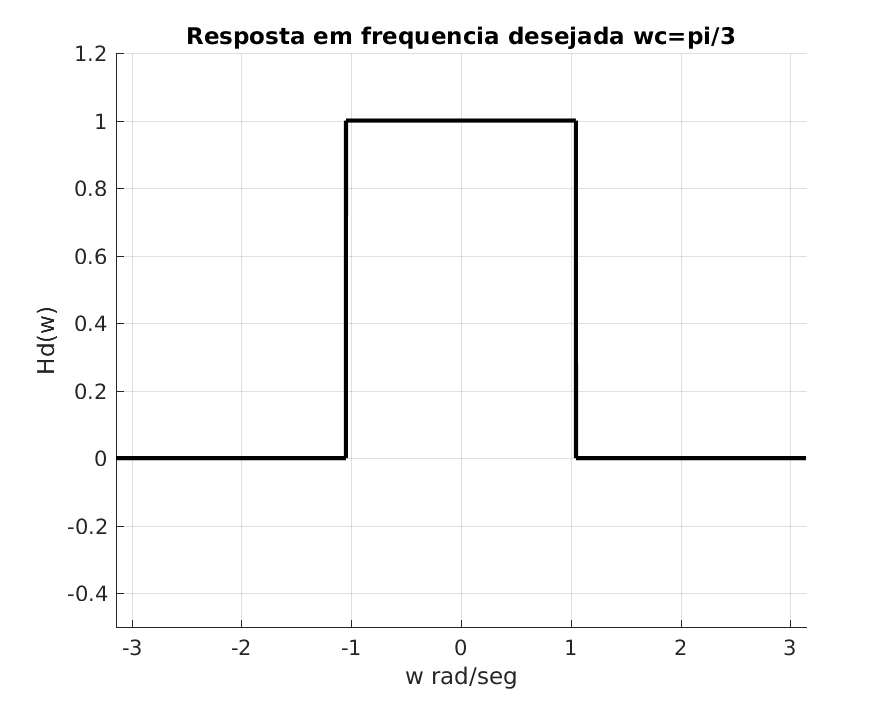
\includegraphics[width=0.4\textwidth]{./figs/idealLowPassFilterResponse.png}}
  \end{subfigure}   
  \begin{subfigure}[]{\label{fig:filter4}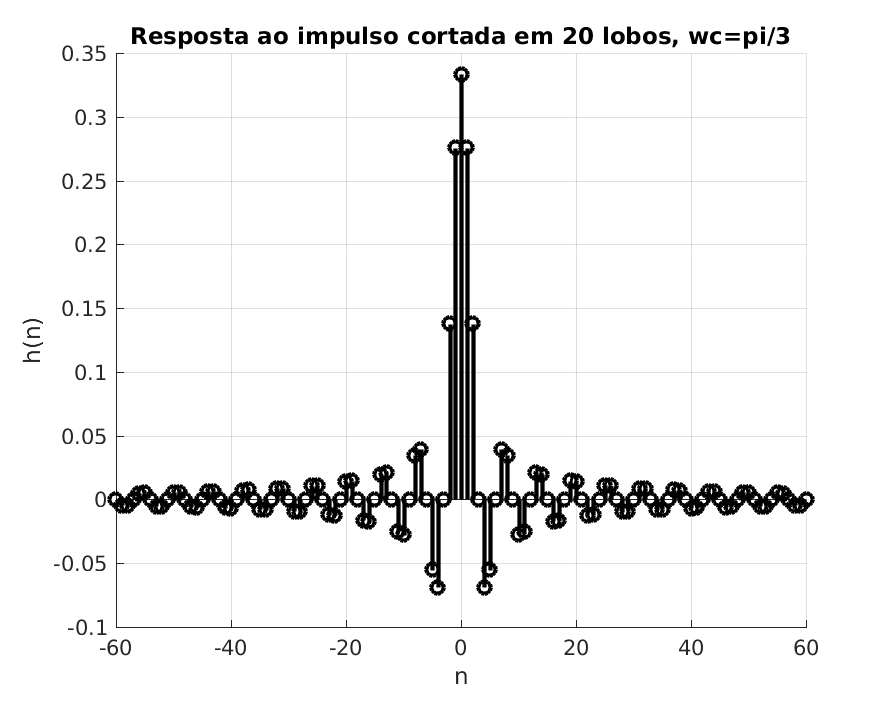
\includegraphics[width=0.4\textwidth]{./figs/infiniteIdealResponse.png}}
  \end{subfigure}

  \caption{Em (a) é observada a resposta ao impulso em frequência ideal de um
    filtro passa-baixas. A frequência de corte projetada é $\omega_c=\frac{\pi}{3}$
    rad/segundos. Em (b) são observados alguns pontos de $h(n)$. Na realidade a sequência é infinita para ambos os lados do eixo.  }

  \label{fig:filtro-passa-baixas-ideal-freq}
\end{figure}

Pode ser observado que além da resposta ser infinita, ela é não causal pois
possui termos não nulos para $n < 0$. Ou seja, o sistema precisaria começar a
responder antes mesmo que a entrada impulso fosse aplicada. Fica claro que a
realização de tal filtro é impossível. Notando que a forma de onda de $h(n)$ é
composta por lobos positivos e negativos, a técnica de janela busca aproximar o
filtro ideal ao limitar $h(n)$ a um número finito de pontos não nulos, de forma
a manter um número inteiro de lobos simétricos. Além disso, $h(n)$ precisa ser
deslocado para a direita caso o objetivo seja um filtro fisicamente realizável. 

A Figura \ref{fig:filtro-passa-baixas-3-lobos} mostra o filtro e a resposta em
frequência obtidos caso a resposta ideal seja cortada com o lobo central e mais
dois lobos simétricos.  A Figura \ref{fig:filtro-passa-baixas-1-lobo} mostra o
filtro e a resposta em frequência obtidos caso mantenha-se somente o lobo
central.  Nota-se que no primeiro caso são necessários 18 valores, enquanto no
segundo apenas 6. Por outro lado, a resposta em frequência no primeiro caso se
aproxima melhor do filtro passa-baixas ideal. Nota-se que há um compromisso que
precisa ser feito entre a qualidade do filtro e a quantidade de memória e
processamento necessários para implementar o filtro.

Para efeito de comparação, a Figura \ref{fig:filtro-passa-baixas-mais-curto}
mostra o mesmo projeto aplicado para a frequência de corte
$\omega_c=\frac{\pi}{10}$. Nota-se que uma frequência de corte mais baixa requer
uma quantidade de pontos não nulos no filtro maior que aquela vista na Figura
\ref{fig:filtro-passa-baixas-3-lobos}.

\begin{figure}[!htb]
  \centering
  \begin{subfigure}[]{\label{fig:filter1}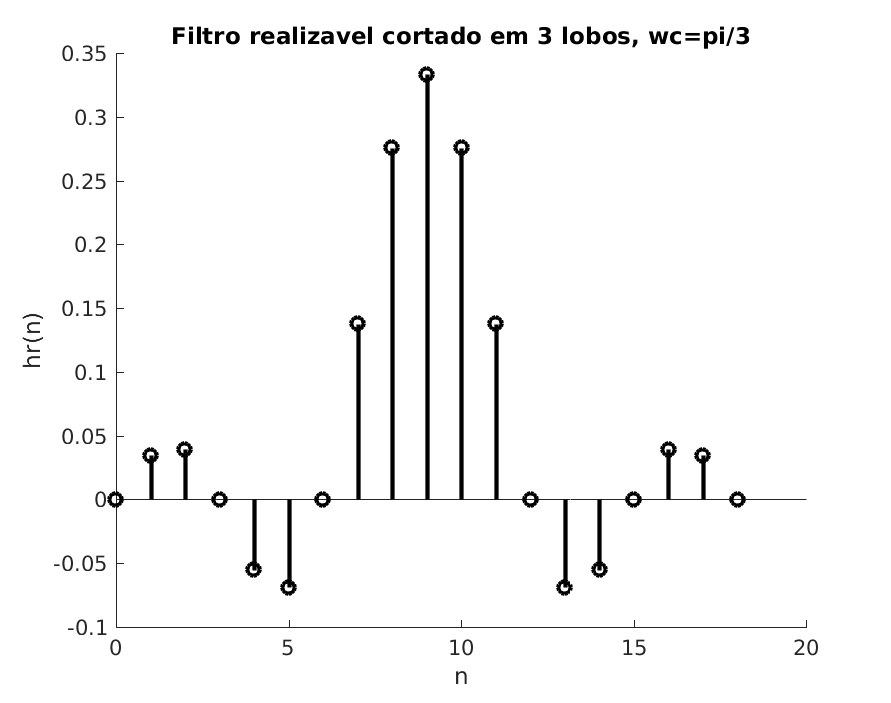
\includegraphics[width=0.4\textwidth]{./figs/realizableFilter3L3.png}}
  \end{subfigure}   
  \begin{subfigure}[]{\label{fig:filter2}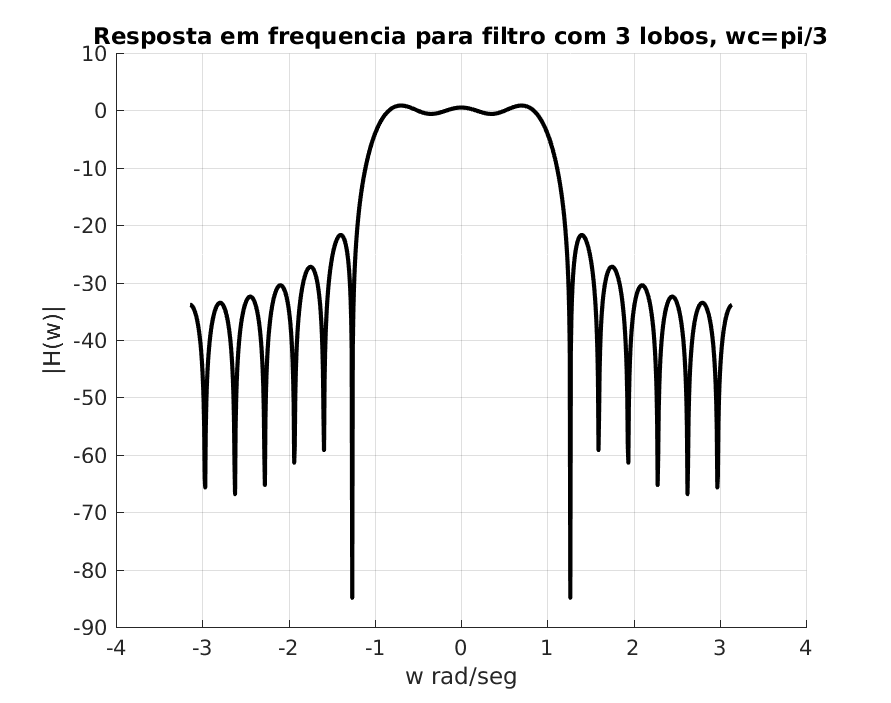
\includegraphics[width=0.4\textwidth]{./figs/filterResponse3L3.png}}
  \end{subfigure}

  \caption{Em (a) é observada a resposta ao impulso do filtro realizável obtido
    cortando-se o lobo principal mais dois lobos para cada lado da resposta
    ideal.  Note que o eixo horizontal foi transladado para permitir uma
    resposta realizável. Em (b) é observada a resposta em frequência obtida com
    esse filtro.  Nota-se que o eixo vertical é mostrado em decibéis.}

  \label{fig:filtro-passa-baixas-3-lobos}
\end{figure}

\begin{figure}[!htb]
  \centering
  \begin{subfigure}[]{\label{fig:filter3}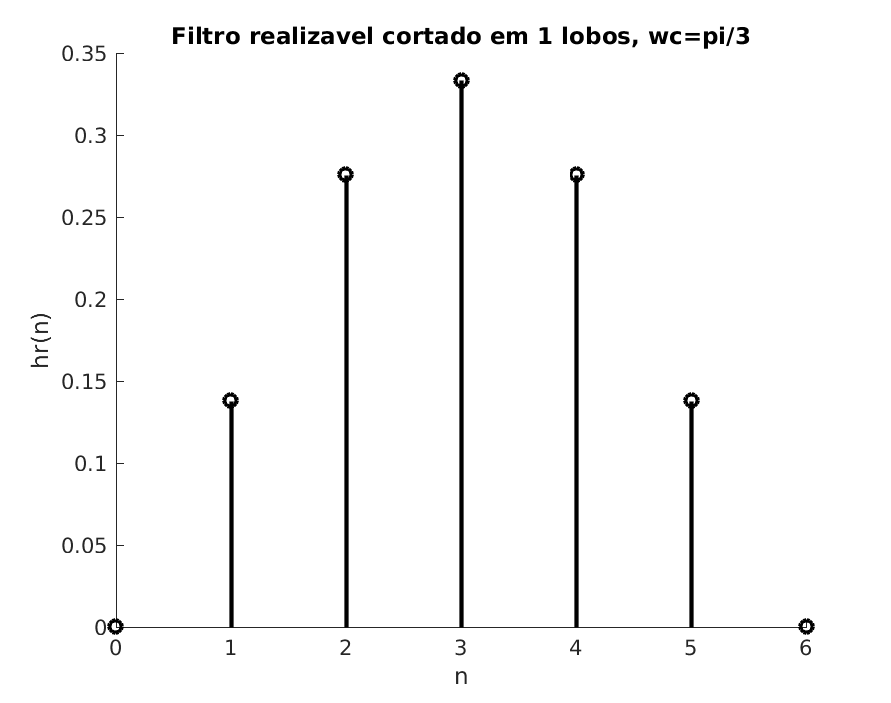
\includegraphics[width=0.4\textwidth]{./figs/realizableFilter1L3.png}}
  \end{subfigure}   
  \begin{subfigure}[]{\label{fig:filter4}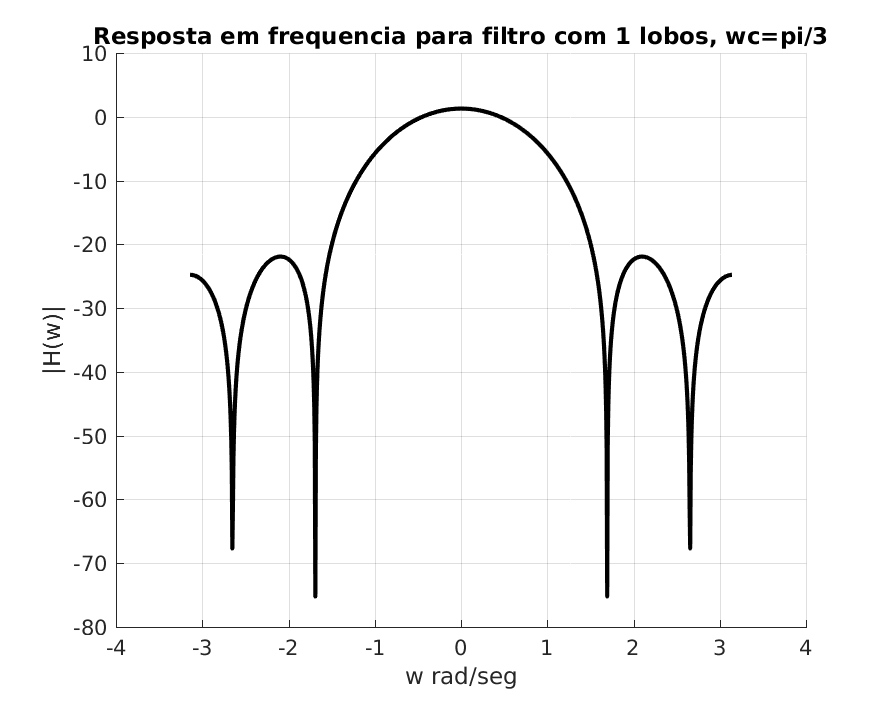
\includegraphics[width=0.4\textwidth]{./figs/filterResponse1L3.png}}
  \end{subfigure}

  \caption{Em (a) é observada a resposta ao impulso do filtro realizável obtido
  cortando-se o lobo principal somente. Em (b) é observada a resposta em
frequência obtida com esse filtro.}

  \label{fig:filtro-passa-baixas-1-lobo}
\end{figure}

\begin{figure}[!htb]
  \centering
  \begin{subfigure}[]{\label{fig:filter3}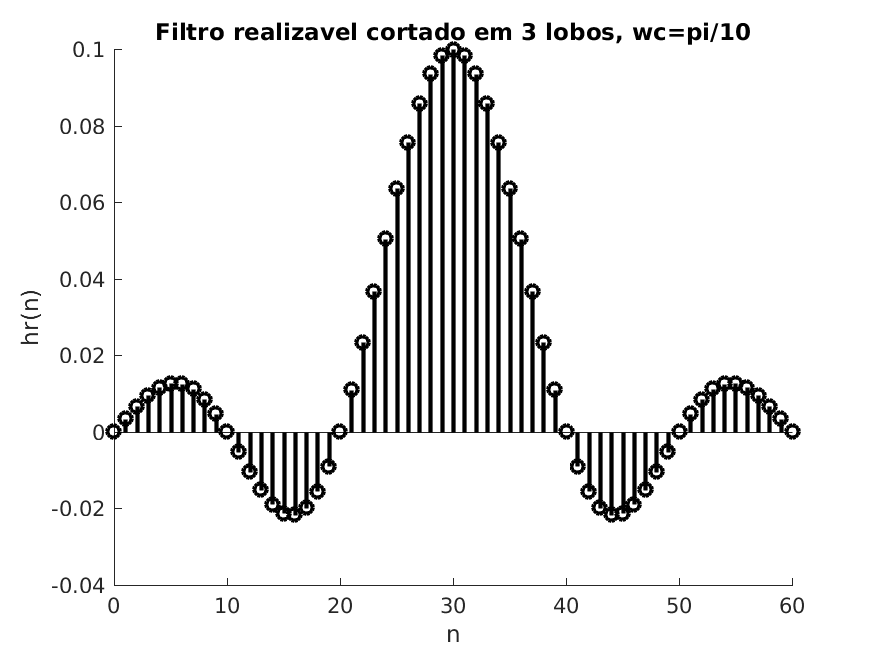
\includegraphics[width=0.4\textwidth]{./figs/realizableFilter3L10.png}}
  \end{subfigure}   
  \begin{subfigure}[]{\label{fig:filter4}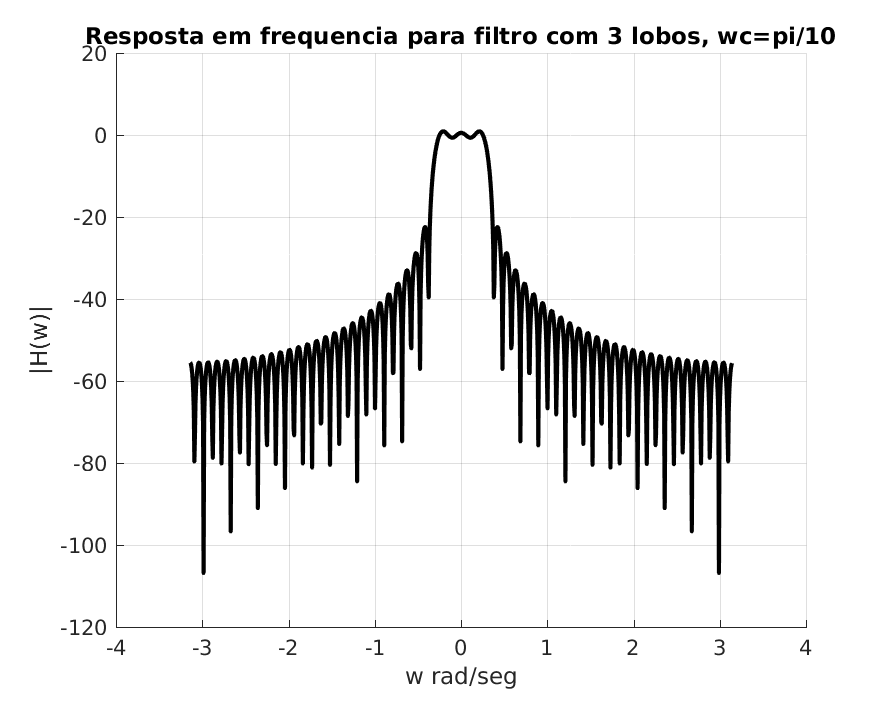
\includegraphics[width=0.4\textwidth]{./figs/filterResponse3L10.png}}
  \end{subfigure}

  \caption{Filtro projetado com 3 lobos e frequência de corte
  $w_c=\frac{\pi}{10}$.}

  \label{fig:filtro-passa-baixas-mais-curto}
\end{figure}

